%%%%%%%%%%%%%%%%%%%%%%%%%%%%%%%%%%%%%%%%%
% Beamer Presentation
% LaTeX Template
% Version 1.0 (10/11/12)
%
% This template has been downloaded from:
% http://www.LaTeXTemplates.com
%
% License:
% CC BY-NC-SA 3.0 (http://creativecommons.org/licenses/by-nc-sa/3.0/)
%
%%%%%%%%%%%%%%%%%%%%%%%%%%%%%%%%%%%%%%%%%

%----------------------------------------------------------------------------------------
%	PACKAGES AND THEMES
%----------------------------------------------------------------------------------------

\documentclass{beamer}

\mode<presentation> {

% The Beamer class comes with a number of default slide themes
% which change the colors and layouts of slides. Below this is a list
% of all the themes, uncomment each in turn to see what they look like.

%\usetheme{default}
%\usetheme{AnnArbor}
%\usetheme{Antibes}
%\usetheme{Bergen}
%\usetheme{Berkeley}
%\usetheme{Berlin}
%\usetheme{Boadilla}
%\usetheme{CambridgeUS}
\usetheme{Copenhagen}
%\usetheme{Darmstadt}
%\usetheme{Dresden}
%\usetheme{Frankfurt}
%\usetheme{Goettingen}
%\usetheme{Hannover}
%\usetheme{Ilmenau}
%\usetheme{JuanLesPins}
%\usetheme{Luebeck}
%\usetheme{Madrid}
%\usetheme{Malmoe}
%\usetheme{Marburg}
%\usetheme{Montpellier}
%\usetheme{PaloAlto}
%\usetheme{Pittsburgh}
%\usetheme{Rochester}
%\usetheme{Singapore}
%\usetheme{Szeged}
%\usetheme{Warsaw}

% As well as themes, the Beamer class has a number of color themes
% for any slide theme. Uncomment each of these in turn to see how it
% changes the colors of your current slide theme.

%\usecolortheme{albatross}
%\usecolortheme{beaver}
%\usecolortheme{beetle}
%\usecolortheme{crane}
%\usecolortheme{dolphin}
%\usecolortheme{dove}
%\usecolortheme{fly}
%\usecolortheme{lily}
%\usecolortheme{orchid}
%\usecolortheme{rose}
%\usecolortheme{seagull}
%\usecolortheme{seahorse}
%\usecolortheme{whale}
%\usecolortheme{wolverine}

%\setbeamertemplate{footline} % To remove the footer line in all slides uncomment this line
%\setbeamertemplate{footline}[page number] % To replace the footer line in all slides with a simple slide count uncomment this line

%\setbeamertemplate{navigation symbols}{} % To remove the navigation symbols from the bottom of all slides uncomment this line
}

\usepackage{graphicx} % Allows including images
\usepackage{booktabs} % Allows the use of \toprule, \midrule and \bottomrule in tables
\usepackage{caption}
\usepackage[english,russian]{babel}
\usepackage[utf8x]{inputenc}
%----------------------------------------------------------------------------------------
%	TITLE PAGE
%----------------------------------------------------------------------------------------

\title[Оптимизация спайковых нейронных сетей]{Оптимизация спайковых нейронных сетей} % The short title appears at the bottom of every slide, the full title is only on the title page

\author{Алексей Чернышев} % Your name
\institute[BMSTU] % Your institution as it will appear on the bottom of every slide, may be shorthand to save space
{
Аспирант РК 6\\
Научный руководитель:\\ д.ф.-м.н Анатолий Павлович Карпенко\\
\medskip
МГТУ им. Н.Э. Баумана \\ % Your institution for the title page
\medskip
\textit{alexey.chernushev@gmail.com} % Your email address
}
\date{\today} % Date, can be changed to a custom date

\begin{document}

\begin{frame}
\titlepage % Print the title page as the first slide
\end{frame}

\begin{frame}
\frametitle{Обзор} % Table of contents slide, comment this block out to remove it
\tableofcontents % Throughout your presentation, if you choose to use \section{} and \subsection{} commands, these will automatically be printed on this slide as an overview of your presentation
\end{frame}

%----------------------------------------------------------------------------------------
%	PRESENTATION SLIDES
%----------------------------------------------------------------------------------------

%------------------------------------------------
\section{Динамические нейронные сети} % Sections can be created in order to organize your presentation into discrete blocks, all sections and subsections are automatically printed in the table of contents as an overview of the talk
%------------------------------------------------

\subsection{Обзор} % A subsection can be created just before a set of slides with a common theme to further break down your presentation into chunks


\begin{frame}
\frametitle{Динамические нейронные сети}
Динамические нейронные сети, также известные как ``вычислительные резервуары'', в зависимости от рабочей формы сигнала делятся на два вида:
\begin{enumerate}
\item Echo State Networks \cite{jaeger} -- непрерывный сигнал\\
\begin{itemize}

\item Являются логическим продолжением идей классических нейронных сетей (нейрон Маккалока-Питтса)
\item Даже на современных компьютерах можно симулировать только небольшие нейронные сети на небольших данных (высокая связность)

\end{itemize}
\item Liquid State Machines \cite{lsm} -- пульсирующий (спайковый) сигнал
\begin{itemize}
\item Биологически инспирированные нейронные сети во многом повторяют динамику настоящих нейронов
\item Спайковая форма сигнала позволяет оптимизировать вычисления динамики сети (Событийное моделирование)
\end{itemize}

\end{enumerate}
\end{frame}

\begin{frame}
\frametitle{Динамические нейронные сети: основные свойства}
\begin{itemize}
\item Нелинейная хаотичная динамика, может быть интересна с т.з. вычислительных способностей сети
\item Специфичное обучение весов сети, как правило обучение без учителя
\item Большой набор гиперпараметров, даже если не включать веса синапсов
\end{itemize}
\end{frame}
%------------------------------------------------
\begin{frame}
\begin{figure}
   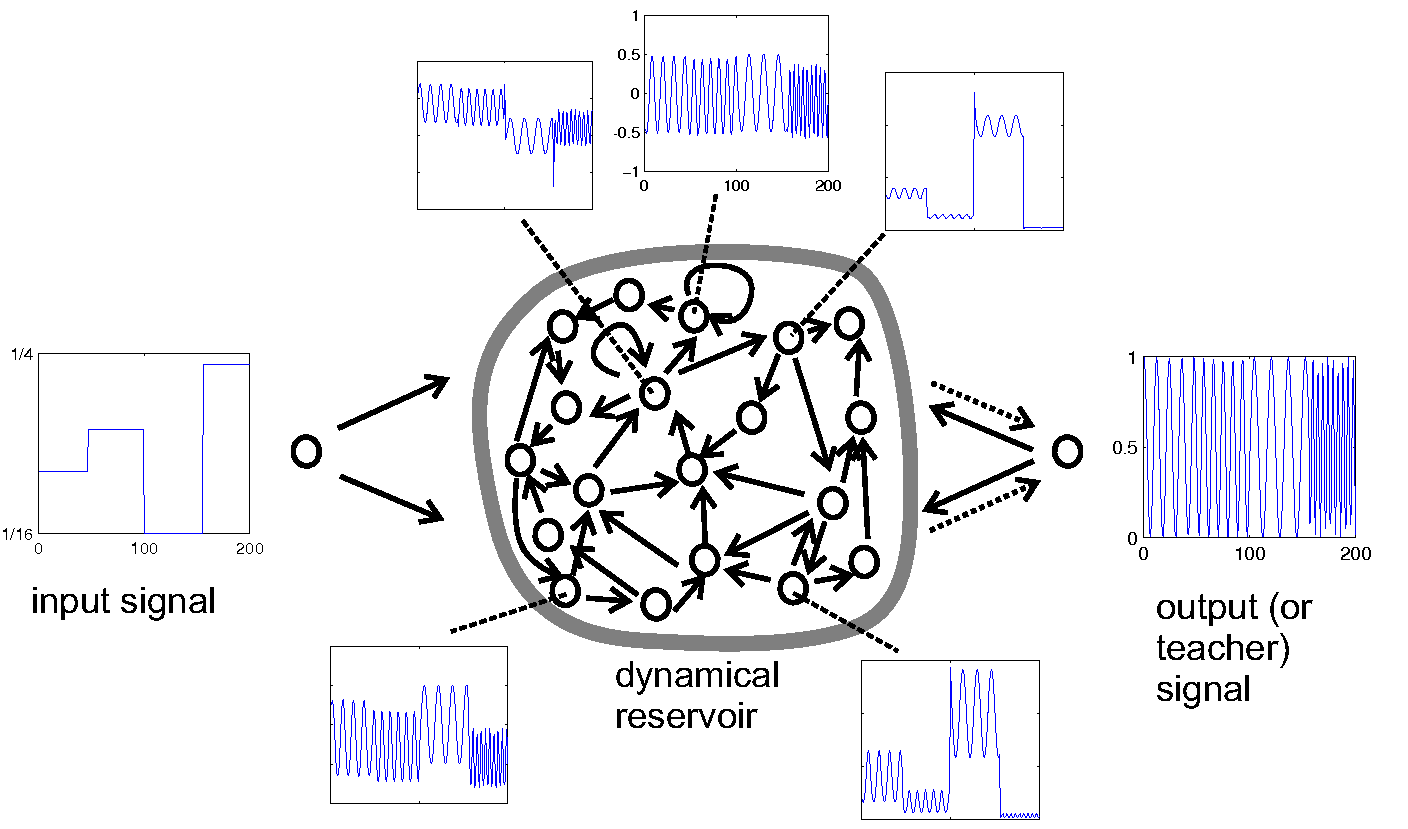
\includegraphics[scale=0.6]{FreqGenSchema.png}
\end{figure}
\hspace*{5pt}\hbox{\scriptsize Источник:\thinspace{\scriptsize\itshape Herbert Jaeger (2007) Echo state network. Scholarpedia, 2(9):2330}}\\

В сети происходит разложение сигнала на составляющие (например частотные)

\end{frame}

\subsection{Проблемы} 


\begin{frame}
\frametitle{Основные проблемы}
Проблемы:
\begin{itemize}
\item Сложная система с множеством гиперпараметров
\item Нет общепринятых функционалов качества работы таких сетей
\item Невыводимые производные функционала качества
\item Вычисление, а особенно обучение, требовательно к ресурсам
\end{itemize}
\end{frame}

%------------------------------------------------
\section{Практика}
\subsection{Функционал качества}

\begin{frame}
\frametitle{Функционал качества}
Введена метрика которая позволяет оценить качество сепарабельности временных рядов для их классификация на основе соотношения Фишера\\
Применение такой метрики происходит в три этапа:

\begin{itemize}
\item Сглаживание пульсирующей формы сигнала
\item Применения ядра, который показывает схожесть двух сигналов
\item Вычисление соотношения Фишера: межклассовая ковариация деленная на внутриклассовую
\end{itemize}

\end{frame}

\begin{frame}
\frametitle{Функционал качества}
\begin{block}{Сглаживающий фильтр}
	\begin{equation}
		\kappa(t)=e^{-\frac{t}{\tau}}
	\end{equation}
\end{block}

\begin{block}{Ядро}
	\begin{equation}
		K_{ij} = \int_{t_{0}}^{t_{1}} \frac{Z^{i}(t)Z^{j}(t)}{|Z^i(t)||Z^j(t)|}dt
	\end{equation}
\end{block}
\begin{block}{Соотношение Фишера}
	\begin{equation}
		F=\frac{tr(S_{B}^{K})}{tr(S_{W}^{K})}
	\end{equation}
\end{block}

\end{frame}


\subsection{Байесовская оптимизация} 
\begin{frame}
\frametitle{Оптимизация функционала качества}
Теория Ресурсоёмкой Глобальной Оптимизации (\textit{Expesnive Global Optimization}\cite{ego-jones}) оказывается очень кстати в подобных задачах и решает проблему: \\
\begin{itemize}
\item За минимальное количество вычислений найти максимум ``чёрного ящика'' -- критерия качества системы.
\end{itemize}
Подобное требование достигается при помощи перевода акцента на суррогатную модель заменяющую исходную функцию. Вычисление точки такой модели является дешевым с т.з. ресурсов компьютера.
\end{frame}

\begin{frame}
\frametitle{Оптимизация функционала качества}
Суррогатная модель задается:
\begin{itemize}
\item Ядром, которое определяет степень гладкости функции
\item Критериальная функция (\textit{Acquisition function})
\end{itemize}
\begin{figure}
   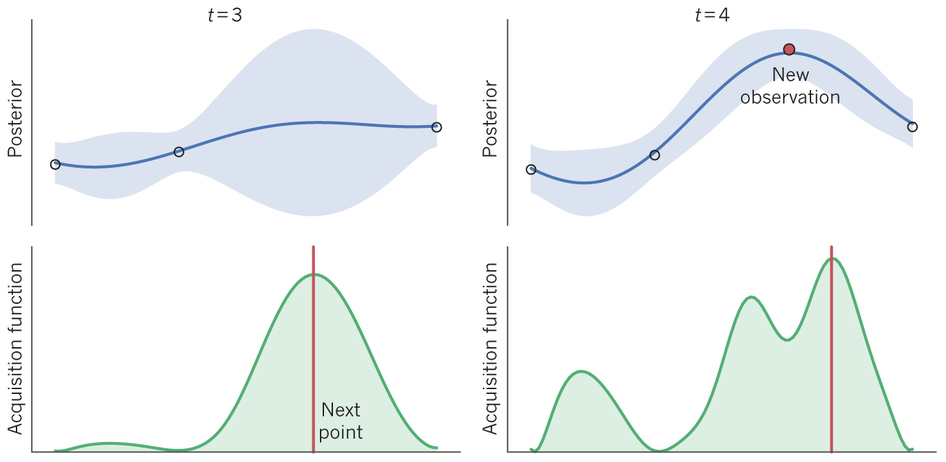
\includegraphics[scale=0.25]{bo.jpg}
\end{figure}
\hspace*{5pt}\hbox{\scriptsize Источник:\thinspace{\scriptsize\itshape Ghahramani Z. Probabilistic machine learning and artificial intelligence}}\\
\end{frame}

\begin{frame}
\frametitle{Оптимизация функционала качества}
Сила рекуррентных связей против качества системы $log(F)$
\begin{figure}
   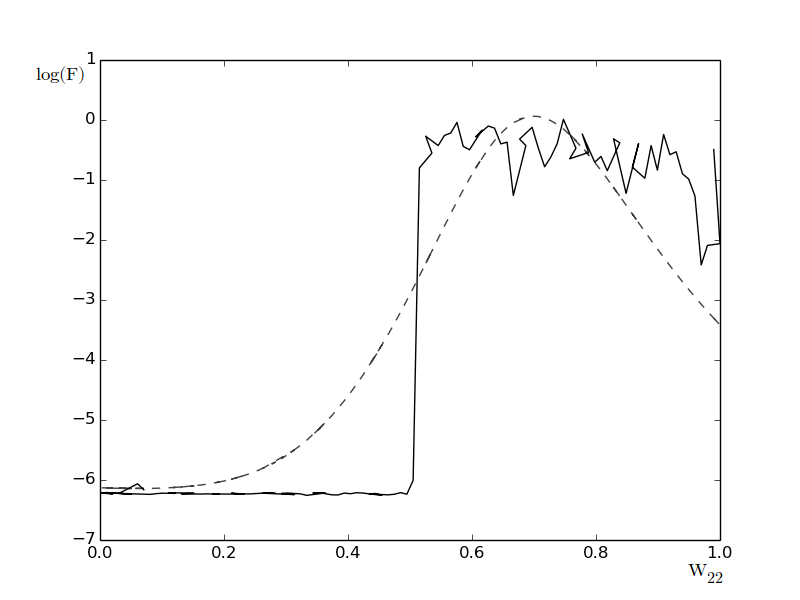
\includegraphics[scale=0.25]{rec_weights_fig.png}
\end{figure}
\end{frame}


\section{Итоги}
\subsection{Проделанная работа и публикации}
\begin{frame}
\frametitle{Итоги}
Проделана работа:
\begin{itemize}
\item Создание методики оптимизации динамических нейронных сетей
\item Создана инфраструктура для экспериментов
\end{itemize}
Публикации за год:
\begin{itemize}
\item {\scriptsize Карпенко А. П., Кострубин М. С., Чернышев А. С. Эффективность классификации многомерных временных рядов с помощью шейплетов. Наука и образование 2015 }
\item {\scriptsize Чернышев А.С., Байесовская оптимизация параметров спайковой нейронной сети для решения задачи классификации временных рядов,  Научно практическая конференция НЕЙРОИНФОРМАТИКА 2016 //Москва, \textit{в процессе ревью} } 
\item {\scriptsize  Chernyshev A.S., Bayesian Optimization of Spiking Neural
Network Parameters to Solving the Time Series
Classification Task, FIERCES ON BICA 2016 //Moscow \textit{in review process} }
\end{itemize}
\end{frame}



\begin{frame}
\frametitle{Ссылки}
\footnotesize{
\begin{thebibliography}{99} % Beamer does not support BibTeX so references must be inserted manually as below
\bibitem{jaeger} Jaeger H. Short term memory in echo state networks. – GMD-Forschungszentrum Informationstechnik, 2001.
MLA	
\bibitem{lsm} Natschläger T., Maass W., Markram H. The" liquid computer": A novel strategy for real-time computing on time series //Special issue on Foundations of Information Processing of TELEMATIK. – 2002. – Т. 8. – №. LNMC-ARTICLE-2002-005. – С. 39-43.
\bibitem{ego-jones} Jones, D. R., Schonlau, M., \& Welch, W. J. (1998). Efficient global optimization of expensive black-box functions. Journal of Global optimization, 13(4), 455-492.

\end{thebibliography}
}
\end{frame}

%------------------------------------------------

\begin{frame}
\Huge{\centerline{Спасибо за внимание}}
\end{frame}

%----------------------------------------------------------------------------------------

\end{document} 